% flavour text, presentation of the problem, may contain images and quotes
% image:
%\begin{figure}[h]
%\center\includegraphics[width=0.3\textwidth]{name.png}
%\end{figure}

\problemname{Buildings}

As a traveling salesman in a globalized world, Alan has always moved a lot.
He almost never lived in the same town for more than a few years until his heart yearned for a different place.
However, this newest town is his favorite yet - it is just so colorful.
Alan has recently moved to Colorville, a smallish city in between some really nice mountains.
Here, Alan has finally decided to settle down and build himself a home - a nice big house to call his own.

In Colorville, many people have their own houses - each painted with a distinct pattern of colors such that no two houses look the same.
Every wall consists of exactly $n \times n$ squares, each painted with a given color (windows and doors are also seen as unique ``colors''). 
The walls of the houses are arranged in the shape of a regular $m$-gon, with a roof on top.
According to the deep traditions of Colorville, the roofs should show the unity among Colorvillians, so all roofs in Colorville have the same color.

\begin{figure}[h]
\begin{center}
    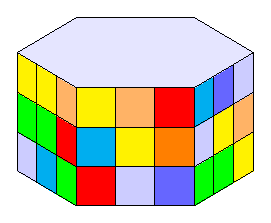
\includegraphics[width=0.5\textwidth]{pic.pdf}
\end{center}
    \caption{Example house design for $n = 3$, $m=6$.}
\end{figure}

Of course, Alan wants to follow this custom to make sure he fits right in.
However, there are so many possible designs to choose from.
Can you tell Alan how many possible house designs there are?
(Two house designs are obviously the same if they can be translated into each other just by rotation.)

\section*{Input}
The input consists of:
\begin{itemize}
	\item one line with three integers $n$, $m$, and $c$, where
	\begin{itemize}
		\item $n$ ($1\leq n\leq 500$) is the side length of every wall, i.e. every wall consists of $n \times n$ squares;
		\item $m$ ($3\leq m\leq 500$) is the number of corners of the regular polygon;
		\item $c$ ($1\leq c \leq 500$) the number of different colors.
	\end{itemize}
\end{itemize}

%The input consists of one line with three integers $n$ ($1\leq n\leq 500$), $m$ ($3\leq m\leq 500$) and $c$ ($1\leq c \leq 500$), where Alan's house should have the shape of a regular $m$-gon with every wall consisting of $n \times n$ squares with each square colored in one of $c$ possible colors.

\section*{Output}
% detailed description of the output format

Output $s$ where $s$ is the number of possible different house designs.
Since $s$ can be very large, output $s \mod (10^9 + 7)$.
